\chapter{Experimentation environment}
\label{cha:des}

Experiments on \ac{BGP} are not applicable on the actual Internet, for this
reason different studies show their results using a simulated environment~\cite{griffin2001experimental}
or emulations executed on a testbed~\cite{milani2020improving}.
In the simulations the majority of the studies use small graphs and each node
of the graph simulate the behaviour of a \ac{BGP} speaker.

For this reason I designed an experimentation system that permits to create and execute
different environments simulating a \ac{BGP} network and then study the sequence
of events as an output.
A schema of this system is presented in \Cref{fig:exp_sketch}.

\begin{figure}[ht]
    \centering
    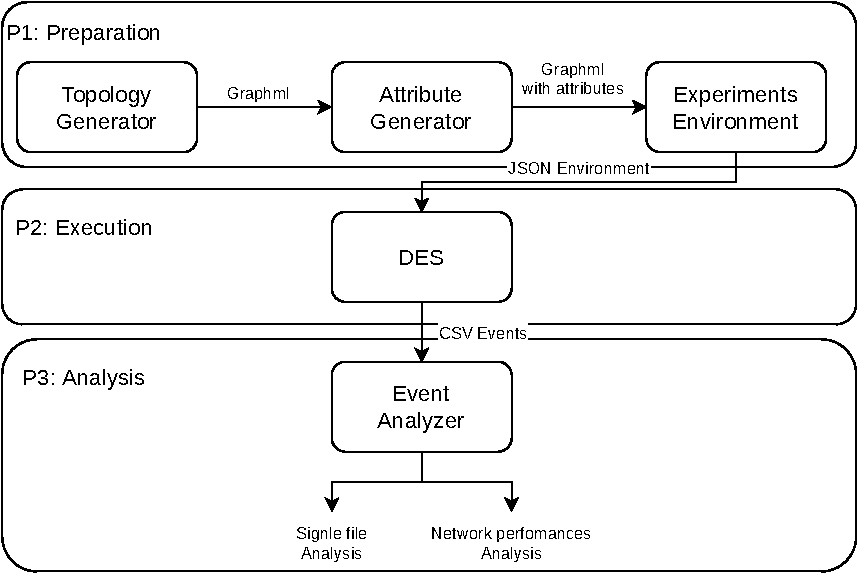
\includegraphics[scale=0.75]{images/toolchain.pdf}
    \caption{Sketch of the experimentation system.}
    \label{fig:exp_sketch}
\end{figure}

Through this system, \Cref{fig:exp_sketch}, is possible to simulate networks
of thousands of nodes, the only limit is given by the computational power where
the software is executed.
All the parts of it are published and documented
online\footnote{\href{https://github.com/tiamilani/BGPFSM}{GitHub repository}}.
All experiments has been repeated multiple times to ensure that the results
has not been biased by random variation of the environment.

All the three macro area of the system can be executed separately and automated
with more elaborate scripts that points to reduce the human interaction with the
software.
Is also possible to execute multiple experiments at the same time, using
\textit{parallel}, in order to overcome the single thread limitation of the
\ac{DES}~\cite{Tange2011a}.
All this scripts are available online with the core of the tool chain.

The three parts that compose the system can be summarized as follow:
\begin{itemize}
		\item \textbf{\textit{Preparation}:} The mandatory material for the
				simulation is created and configured in this phase in order to
				pass to the next phase a complete environment;
		\item \textbf{\textit{Execution}:} This phase is composed only by the
				\ac{DES} that takes as input an environment that describe the
				properties that the network has to respect to evolve, giving as
				output a file that contains all the events triggered;
		\item \textbf{\textit{Analysis}:} This is the last phase, which goal
				is to analyze the output of an experiment or a set of experiments
				to produce plots or \textit{CSV} files that summarize some
				properties of the network evolution.
\end{itemize}

\section{Environment preparation}
\label{sec:exp_prep}

All the experiments executed relay on an environment that contains all
the information necessary for the \ac{DES} to make the network evolve.
First of all, is mandatory to create a topology that represent the network
of \acp{AS} which is used by the simulator.
Then, could be necessary to configure
different parameters, for example, \ac{MRAI} on the links, the
\ac{RFD} mechanism or other properties of the node.
Finally, is possible to insert the reference to the graph inside the file that
describes the environment with all the other properties of it, like the delay
on the links or the \ac{RNG} initial values.
After that, is possible to pass this file to the \ac{DES} that will execute
the experiments.

\subsection{BGP Topology generation}
\label{subsec:exp_topology_generation}

To store all the topological information that represent a \ac{BGP} graph I use
the \textit{graphml} standard.
I developed two components that can be used to generate and populate the graph
file.
The first one is the graph generator, through it is possible to obtain graphml
files with the required topology. For the time being is possible to generate
clique or Internet-like topologies.
The output graph is a directed graph that contains the required number of nodes
and all the edges.
The second software that is possible to use is the \q{Attribute Generator}, this
tool is an agglomerate of small gadgets which goal is to add some properties to
the graph, those properties could be for example the \ac{RFD} mechanism for
the nodes or the \ac{MRAI} with a explicit distribution on the edges.

The model used to represent the \ac{BGP} network is a directed graph \graph,
where every edge in \nodeset represent a single \ac{AS} and every edge in
\edgeset model the relation between two \acp{AS} \(i,j\).
The properties that can be defined for every node are the following:
\begin{itemize}
		\item \textit{type \(\{T,M,C,CP\}\)}: This attribute defines the type
				of the node in the Internet-like topologies, tier-1,
				mid-level, customer, or content provider;
		\item \textit{centrality}: The centrality attributed to the node;
		\item \textit{destinations}: If the node shares some destination can
				be listed using this attribute, a node can also don't share
				any destination;
		\item \textit{\ac{RFD}}: This attribute defines the parameter used
				to configure the \ac{RFD} function of the node.
\end{itemize}

For every \((i,j)\) in \edgeset where \(i,j \in \nodeset\) the possible properties
are:
\begin{itemize}
		\item \textit{delay}: Is possible to define a specific delay distribution
				that would be used only on the link \(i,j\);
		\item \textit{policy}: This attribute defines the relationship between
				\(i\) and \(j\) and will be used to check if a message can
				be transmitted on the link, policies are encoded using the
				algebra described in~\cite{daggitt2018rate};
		\item \textit{\ac{MRAI}}: This attribute describe the \ac{MRAI} value
				that would be used by \(i\) with the neighbour \(j\).
\end{itemize}

An extract from a graphml file is showed in Code~\ref{lst:graph_example}.
\lstcaptionname{Code}
\begin{lstlisting}[language=graphml, caption=Graph example, label=lst:graph_example]
 <node id="0">
      <data key="d0">10.0.0.0/24</data>
 </node>
 <edge source="2" target="5">
     <data key="d2">2, 2, 2</data>
 </edge>
\end{lstlisting}

\subsection{Environment definition}
\label{subsec:exp_environments_definition}

The environment where the network evolve is defined with a \textit{JSON}
file that contains all the properties used by the \ac{DES}.
Inside the environment are also defined the values to initialize the \ac{RNG}
so that every experiment is completely reproducible.

Is possible to define in the environment two different types of evolution:
\begin{itemize}
    \item \textbf{\textit{Continuous evolution}}: In this category all the nodes
    that contains at least one destination will continuously share and retrieve
    the destination accordingly with the distributions defined in the environment;
    \item \textbf{\textit{Signaling evolution}}: Is possible to define a precise
    signal that should be followed by the nodes that contain a destination, for
    example, the signal \q{AWA} defines that there will be an announce followed by
    a withdraw and then another announce.
\end{itemize}

Thanks to the \textit{JSON} format is possible to have a high grade of
freedom and vectors of properties.
Those vectors can contain $n$ objects that describe that property, but in each
run just one of them can be used.
Each run is composed by a combination of one object from each vector.
For example, with \num{5} different possible seeds and \num{3} different
delays, the total number of runs combinations is \num{15}, as shown in Code
\ref{lst:environment_example}.
%If a property has only one object, then, this object will be used in every
%combination.
%If all the properties have only one object then the environment describes only
%a single run.
A unique identifier is associated to every possible run, through it is possible
to execute specific experiments.

\lstcaptionname{Code}
\begin{lstlisting}[language=json, caption=Environment example with \num{15} possible runs, label=lst:environment_example]
"simulation" : {
    // seed(s) to initialize RNG
    "seed" : [0, 1, 2, 3, 4],
    ....
    // Multiple withdraw distributions
    "withdraw_dist": [{"distribution": "unif", "min": 5, "max": 10, "int": 0.1},
                      {"distribution": "unif", "min": 8, "max": 10, "int": 0.1},
                      {"distribution": "unif", "min": 2, "max": 3, "int": 0.1}],
    ....
}
\end{lstlisting}

%In the environment is possible to define also the processing time, this time is used
%inside each \ac{BGP} node to simulate the processing of information or the evaluation
%of a packet.
%The \textit{delay} parameter describes the default delay on the edges,
%The links are FIFO so there is no reordering of messages in the same link,
%no messages are lost during transmissions.
%That because it was out of the scope of this thesis to study the evolution
%of the protocol with packet loss, but it could be in the future works.

I defined multiple standard environments to study different
properties and behaviours of \ac{BGP} network.

\subsubsection{Clique environment}
\label{subsec:clique_env}

One of the special environment that I defined in my experiments uses clique
graphs of different dimensions, an example of the clique graph is given in
\Cref{fig:clique_topology}.
This environment points to produce a high load of messages that each node has
to process in order to take the best decision on how to reach the single
destination distributed.

The only node that shares a destination is the node \q{\textit{d}}, the node
\num{0} will then spread the knowledge to the whole network, and the node
\q{\textit{x}} will act as a black hole for all the possible paths
that the node \num{5} will share.

This topology is used to enforce the \textit{Path exploration} problem, it also
gives the possibility to study how \ac{BGP} parameters can influence the messages
distribution in stressful cases.

\subsubsection{Fabrikant environment}
\label{subsec:fabrikant_env}

Another interesting case to test the path exploration problem is the one
presented in~\cite{fabrikant2011there}.
In that study, Fabrikant et al. presents how particular \ac{MRAI} setting could
make the network converge with an exponential behaviour. The continuous decision
change in the nodes \ac{RIB} is the cause of the problem.
I used the basic example of their study to investigate how the choice of \ac{MRAI}
is fundamental for the network convergence.
An example of the network used is presented in \Cref{fig:fabrikant_topology}.

%The path exploration problem is caused by the delay on the \num{0}-\num{2}
%edge. The node \num{2} will receive the destination through node \num{1}, after a small amount
%of time the network will converge to the best path (without using the backup links).
%But, after a while, node \num{2} will receive the network also through node \num{0}
%and it will prefer this new path, provoking then the reconfiguration of all
%the other nodes that will use the backup links for a while, announcing their
%new paths.
%A wrong configuration of \ac{MRAI} can provoke the entire exploration of the
%possibility set.

This environment is also used to show how a \ac{BGP} \ac{FSM} would explode
in terms of possible states and edges producing an enormous amount of
output signals from the same input.
This behaviour is presented in \Cref{sec:bgp_fsm_explosion}.

\subsubsection{Internet-like environment}
\label{subsec:internet_like_env}

The last noteworthy environment is the one whose purpose is to simulate the Internet
behaviour.
This has been possible thanks to the study by Elmokashfi et al.~\cite{elmokashfi2010scalability}
and the internet like graph generator present in Networkx \footnote{\href{https://networkx.org/documentation/stable/reference/generated/networkx.generators.internet_as_graphs.random_internet_as_graph.html\#networkx.generators.internet_as_graphs.random_internet_as_graph}{Networkx internet as graph generator}}
(a Python library famous for graph and network studies).
An example with a small set of nodes is presented in \Cref{fig:internet_like_topology}.

The different nodes are coloured accordingly with the node type represented.
The tier one nodes that generate the central clique are coloured in red and
is possible to notice in \Cref{fig:internet_topology_hierarchical} that they are
in the highest levels of the networks.

\section{Discrete Event Simulator}
\label{sec:exp_des}

The second part of the system described in \Cref{fig:exp_sketch} is composed by
the execution of the experiments through the \ac{DES} designed to simulate
\ac{BGP} networks.
I decided to use the \textit{Simpy}\footnote{\href{https://simpy.readthedocs.io/en/latest/index.html}{Simpy website}}
package to instantiate the environment and make it evolve.
This package present an extensive documentation and it has already been used for different
studies, demonstrating its adaptability~\cite{matloff2008introduction,dagkakis2013manpy},
other than an active community.

%I developed the \ac{DES} as a highly modular environment.
%\begin{figure}[h]
%    \begin{center}
%        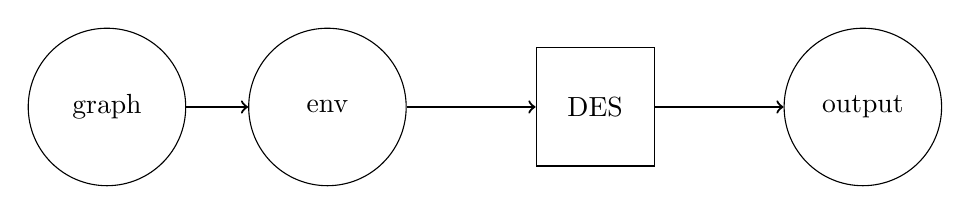
\begin{tikzpicture}[scale=0.2, every node/.style={draw=black,circle,inner sep=0pt}]
    \node [minimum size=2cm] (graph) at (0,0) {graph}; 
    \node [minimum size=2cm] (env) at (14,0) {env};                                    
    \node [rectangle, draw, minimum width=1.5cm,minimum height=1.5cm] (des) at (31,0) {DES};
    \node [minimum size=2cm] (output) at (48,0) {output};                                    
    \draw [thick, ->] (graph) to (env);                                  
    \draw [thick, ->] (env) -- (des);                                 
    \draw [thick, ->] (des) -- (output);                                 
\end{tikzpicture}                                                       

%    \end{center}
%    \caption{DES Experimentation components}
%    \label{fig:des_structure}
%\end{figure}

%In \Cref{fig:des_structure} is possible to see the basic idea behind the simulator.
%The first component needed is a graph, represented by a \textit{graphml} file,
%this file is the descriptor of the network.
%It defines also all the topological information and properties of every single node.
%In Code~\ref{lst:graph_example} is possible to see an example of a \textit{graphml} file,
%it describes that node \num{0} contains a single destination and that the edge
%between nodes \num{2} and \num{5} is controlled by the policy |2, 2, 2| that defines
%a servicer-provider policy.
%The policies are encoded using the convention described in~\cite{daggitt2018rate}.
%In the graph file Is possible to define multiple topological properties, for
%example the \ac{MRAI} value in an edge or the set of parameters that
%controls \ac{RFD}.
%
%The graph is then embedded in the environment file, this is a \textit{JSON} file
%that describes how the environment is characterized.
%Inside of it is possible to define the initial values for the \ac{RNG} so
%that each experiment is replicable.
%In the environment file is also possible to define different properties that
%would be used to make the experiments evolve, for example the distribution that
%will be used for the network delay.
%Is also possible to define multiple values for single properties and decided which
%combination of them to use before the experiment starts.
%There are two possible evolution of the environment that can be used:

The \ac{DES} take as input the \textit{JSON} file that describes all the necessary
information.
Then, it creates an object for each node in the network, respecting
the topological characteristics defined in the \textit{graphml} file.
After the initialization, all the nodes that contain a destination will schedule
the first advertisement to their neighbours.
Given the seeds in the environment file is possible to reproduce the experiments
and obtain the same sequence of events.

At this point, the network can evolve, every event would trigger a reaction by
the nodes that can end up in an other event if necessary.
All the simulated links use a \ac{FIFO} structure, there is no reordering of
the messages and there is no loss of packets.
The nodes evaluates the messages following the arrival order, but is possible
to process only one message at a time.
The simulation run will terminate only if there are no more events scheduled or
if the maximum simulation time is reached.

The \ac{DES} produces a \textit{CSV} output that contains all the events triggered and the
data associated during the evolution of the experiment.
For each event the \ac{DES} will record the exact moment when it happened and
the data concerning the event.
For example for the reception of a message would be registered
the node that received the message and the message itself in plain text.
This \textit{CSV} file is then used for the following part of the tool chain.

\section{Analysis of the events}
\label{sec:exp_output_study}

The last component of the system, \Cref{fig:exp_sketch}, is the analyzer.
This tool goal is to study the sequence of events produced by the \ac{DES} and
process the results.
The input of the analyzer are:
\begin{itemize}
		\item \textit{Events CSVs}: The files that describe the evolution of
				the environment, is possible to analyze multiple files in order
				to produce average results on multiple runs.
		\item \textit{Analysis type \{Single node, Network performances\}}:
				Describes the type of the analysis that is required, is possible
				to analyze a single node evolution or in general the performances
				of the network.
\end{itemize}

In the \textit{Single node} case, is possible to study the evolution of a single
node considering its \ac{RIB}, the input messages and the output messages triggered.
This type of study is used to produce the \ac{FSM} study presented in \Cref{cha:bgp_fsm}.
It permits to produce the \ac{FSM} schema of a node and the output signals
generated by the runs.
The second case, \textit{Network performances}, is used to study the general
evolution of the network in terms of convergence time, number of messages
transmitted etc.
An example of results from this type of study are given in \Cref{cha:bgp_mrai_experiments,cha:bgp_rfd}.

The output of the analyzer are plots and \textit{CSV} files.
The plots represent information that could be simply processed, for example
the \ac{FSM} of a node or the boxplot of the transmitted messages.
The \textit{CSV} files contains information about the experiments that can be
interpreted by other scripts in order to plot more complex evolution or to
correlate multiple experiments.

